%
% Copyright (c) 2012 The NetBSD Foundation, Inc.
% All rights reserved.
%
% This code is derived from software contributed to The NetBSD Foundation
% by Radoslaw Kujawa.
%
% Redistribution and use in source and binary forms, with or without
% modification, are permitted provided that the following conditions
% are met:
% 1. Redistributions of source code must retain the above copyright
%    notice, this list of conditions and the following disclaimer.
% 2. Redistributions in binary form must reproduce the above copyright
%    notice, this list of conditions and the following disclaimer in the
%    documentation and/or other materials provided with the distribution.
%
% THIS SOFTWARE IS PROVIDED BY THE NETBSD FOUNDATION, INC. AND CONTRIBUTORS
% ``AS IS'' AND ANY EXPRESS OR IMPLIED WARRANTIES, INCLUDING, BUT NOT LIMITED
% TO, THE IMPLIED WARRANTIES OF MERCHANTABILITY AND FITNESS FOR A PARTICULAR
% PURPOSE ARE DISCLAIMED.  IN NO EVENT SHALL THE FOUNDATION OR CONTRIBUTORS
% BE LIABLE FOR ANY DIRECT, INDIRECT, INCIDENTAL, SPECIAL, EXEMPLARY, OR
% CONSEQUENTIAL DAMAGES (INCLUDING, BUT NOT LIMITED TO, PROCUREMENT OF
% SUBSTITUTE GOODS OR SERVICES; LOSS OF USE, DATA, OR PROFITS; OR BUSINESS
% INTERRUPTION) HOWEVER CAUSED AND ON ANY THEORY OF LIABILITY, WHETHER IN
% CONTRACT, STRICT LIABILITY, OR TORT (INCLUDING NEGLIGENCE OR OTHERWISE)
% ARISING IN ANY WAY OUT OF THE USE OF THIS SOFTWARE, EVEN IF ADVISED OF THE
% POSSIBILITY OF SUCH DAMAGE.
%
%
% Presentation for NetBSD drivers tutorial for Snow B.V.
%
% TeX layout based on examples provided by Jean-Yves Migeon
%
% The following people provided important suggestions and corrections: 
% Greg Oster, Valery E. Ushakov, S.P. Zeidler
%
% 
\documentclass[dvipsnames,table]{beamer}

\usetheme{Rochester}
\usecolortheme{orchid}

\usepackage{listings}
\usepackage{ucs}
\usepackage[utf8x]{inputenc}
\usepackage{wasysym}
\usepackage[normalem]{ulem}
\usepackage{amsmath}
\usepackage{hyperref}

\setbeamertemplate{navigation symbols}{}
\setbeamertemplate{caption}[numbered]
\setbeamerfont{caption}{size=\scriptsize}
\setbeamercolor{framenote}{bg=NetBSD-orange!25}
\setbeamercolor{rednote}{bg=Red!25}
\setbeamercolor{palette primary}{use=structure,fg=white,bg=NetBSD-orange}
\setbeamercolor{palette secondary}{use=structure,fg=white,bg=NetBSD-orange2}

\setbeamertemplate{itemize item}{\scriptsize\raise1pt\hbox{\donotcoloroutermaths$\blacktriangleright$}}
\setbeamertemplate{itemize subitem}{\tiny\raise1pt\hbox{\donotcoloroutermaths$\bullet$}}
\setbeamertemplate{itemize subsubitem}{\tiny\raise1pt\hbox{\donotcoloroutermaths{--}}}

\setbeamertemplate{enumerate item}{\insertenumlabel.}
\setbeamertemplate{enumerate subitem}{\insertenumlabel.\insertsubenumlabel}
\setbeamertemplate{enumerate subsubitem}{\insertenumlabel.\insertsubenumlabel.\insertsubsubenumlabel}
\setbeamertemplate{enumerate mini template}{\insertenumlabel}

\setbeamercolor{itemize item}{fg=NetBSD-orange, bg=NetBSD-orange}
\setbeamercolor{itemize subitem}{fg=NetBSD-orange, bg=NetBSD-orange}
\setbeamercolor{itemize subsubitem}{fg=NetBSD-orange, bg=NetBSD-orange}

\setbeamercolor{section number projected}{fg=white,bg=NetBSD-orange}
\setbeamercolor{subsection number projected}{fg=white,bg=NetBSD-orange}
\setbeamercolor{button}{bg=NetBSD-orange,fg=white}

\setbeamertemplate{section in toc}[circle]
\setbeamertemplate{subsection in toc}[square]


\definecolor{NetBSD-orange}{RGB}{242,103,17}
\definecolor{NetBSD-orange2}{RGB}{177,76,12}
\hypersetup{colorlinks=true,linkcolor=white,urlcolor=NetBSD-orange}

\setlength{\tabcolsep}{8pt}
\renewcommand{\arraystretch}{1.2}

\newcommand{\nbsdcolor}[1] {
	{\color{NetBSD-orange} #1}
}

\lstset{
   language=C,
   basicstyle=\tiny,
   breaklines=true,
   escapechar=\@,
   commentstyle=\color{NetBSD-orange}
}

\AtBeginSection[]{
%\begin{frame}
%\begin{center}
%\Huge fooo \insertsection
%\end{center}
%\end{frame}
\frame{\sectionpage}

}

\title{Writing NetBSD drivers -- a crash course}

\author{Radoslaw Kujawa -- rkujawa@NetBSD.org}

\institute{The NetBSD Foundation}

\begin{document}

\begin{frame}
\titlepage
\end{frame}

\begin{frame}[allowframebreaks]
\frametitle{Table of Contents}
{
\hypersetup{colorlinks=true,linkcolor=black,urlcolor=NetBSD-orange}
\tableofcontents
}
\end{frame}

\section{Introduction}

\subsection{Hello!}

\begin{frame}
\frametitle{Foo}
\begin{itemize}
	\item EuroBSDcon 2012 -- 4 people attended the tutorial
	\item Writing device drivers is often considered black magic
	\item Reading the {\tt man} pages won't give you the big picture
	\item BSD systems are always in need of new drivers
	\item Device drivers are fun {\Large \smiley}
\end{itemize}
\end{frame}


\subsection{Basic concepts}

\begin{frame}
\frametitle{Basic concepts}
\begin{itemize}
	\item What is a driver anyway?
	\begin{itemize}
		\item The interface between user space and hardware, implemented as a part of the kernel
		\item The NetBSD drivers are written mostly in C
		\item Sometimes they have machine dependent assembler parts, but this is a rare case
	\end{itemize}
	\item What do you need to write a driver?
	\begin{itemize}
		\item C programming skills
		\item Hardware documentation (or the ability to reverse engineer the hardware)
		\item A reference driver implementation will help but is not essential
		\item A NetBSD installation and kernel source, or a cross-build environment (the latter is usually preferred for development of drivers)
		\item A lot of time, coffee and patience {\Large \smiley}
	\end{itemize}
\end{itemize}
\end{frame}

\subsection{}

\begin{frame}
\frametitle{Why is writing the device drivers considered difficult?}
\begin{itemize}
	\item It's not as difficult as you may expect, in fact during this tutorial we'll prove that it's quite easy
	\item You need to think on a very low level
	\begin{itemize}
		\item Good understanding of computer architecture is a must
	\end{itemize}
	\item Often documentation is the main problem -- writing the driver is not possible if you don't understand how the device works
	\begin{itemize}
		\item No access to documentation (uncooperative hardware vendors, vendors out of business)
		\item Documentation is incomplete or plain wrong
		\item Reverse engineering can solve these problems but it's a very time consuming process
	\end{itemize}
\end{itemize}
\end{frame}

\section{The NetBSD driver model}
\subsection{The NetBSD kernel basics}

\begin{frame}
\frametitle{The NetBSD kernel basics}
\begin{itemize}
	\item NetBSD has a classic monolithic UNIX-like kernel - all drivers are running in the same address space
	\item Thanks to the above, communication between drivers and other kernel layers is simple
	\item However, it also means that one badly written driver can affect the whole kernel
	\item Numerous in-kernel frameworks standardise the way drivers are written ({\tt bus\_space}, {\tt autoconf}, etc.) 
\end{itemize}
\end{frame}

\begin{frame}
\frametitle{The NetBSD source directory structure}
\begin{itemize}
	\item We'll only cover parts interesting for a device driver programmer
	\item {\tt src/sys/} - kernel source directory
	\item {\tt src/sys/dev/} - machine-independent device drivers
	\item {\tt src/sys/arch/} - port-specific or architecture-specific parts (such as the low-level system initialisation procedures or machine-dependent drivers)
	\item {\tt src/sys/arch/\$PORTNAME/conf/} - kernel configuration files for a given port

\end{itemize}
\end{frame}

\subsection{Kernel autoconfiguration framework}

\begin{frame}
\frametitle{Kernel autoconfiguration framework - autoconf(9)}
\begin{itemize}
	\item Autoconfiguration is the process of matching hardware devices with an
     appropriate device driver
    \item The kernel message buffer (dmesg) contains information about autoconfiguration of devices
    \item {\tt driver0 at bus0: Foo hardware} 
    \begin{itemize}
    	\item Instance 0 of the driver has attached to instance 0 of the particular bus
		\item Such messages often carry additional bus-specific information about the exact location of the device (like the device and function number on the PCI bus)
	\end{itemize}
    \item {\tt driver0: some message}
    \begin{itemize}
    	\item Additional information about the driver state or device configuration
	\end{itemize}
\end{itemize}
\end{frame}

\begin{frame}[fragile]
\frametitle{Autoconfiguration as seen in the dmesg}
\tiny
\begin{verbatim}
NetBSD 6.99.12 (GENERIC) #7: Fri Oct  5 18:43:21 CEST 2012
        rkujawa@saiko.local:/Users/rkujawa/netbsd-eurobsdcon2012/src/sys/arch/cobalt/compile/obj/GENERIC
Cobalt Qube 2
total memory = 32768 KB
avail memory = 27380 KB
mainbus0 (root)
com0 at mainbus0 addr 0x1c800000 level 3: ns16550a, working fifo
com0: console
cpu0 at mainbus0: QED RM5200 CPU (0x28a0) Rev. 10.0 with built-in FPU Rev. 1.0
cpu0: 48 TLB entries, 256MB max page size
cpu0: 32KB/32B 2-way set-associative L1 instruction cache
cpu0: 32KB/32B 2-way set-associative write-back L1 data cache
mcclock0 at mainbus0 addr 0x10000070: mc146818 compatible time-of-day clock
panel0 at mainbus0 addr 0x1f000000
gt0 at mainbus0 addr 0x14000000
pci0 at gt0
pchb0 at pci0 dev 0 function 0: Galileo GT-64011 System Controller, rev 1
pcib0 at pci0 dev 9 function 0
pcib0: VIA Technologies VT82C586 PCI-ISA Bridge, rev 57
viaide0 at pci0 dev 9 function 1
viaide0: VIA Technologies VT82C586 (Apollo VP) ATA33 controller
viaide0: primary channel interrupting at irq 14
atabus0 at viaide0 channel 0
viaide0: secondary channel interrupting at irq 15
atabus1 at viaide0 channel 1
wd0 at atabus0 drive 0
wd0: <netbsd-cobalt.img>
wd0: 750 MB, 1524 cyl, 16 head, 63 sec, 512 bytes/sect x 1536192 sectors\end{verbatim}
\end{frame}

\begin{frame}
\frametitle{Autoconfiguration as seen in the dmesg}
\begin{center}
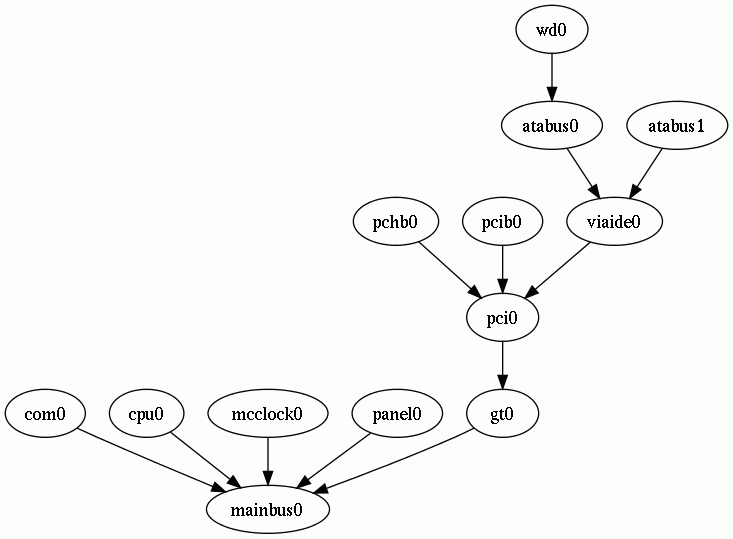
\includegraphics[scale=0.4]{img_cobaltdevices.png}
\end{center}
\end{frame}

\begin{frame}
\frametitle{The {\tt bus\_space(9)} framework}
\begin{itemize}
	\item ``The goal of the {\tt bus\_space} functions is to allow a single
     driver source file to manipulate a set of devices on different system
     architectures, and to allow a single driver object file to manipulate a
     set of devices on multiple bus types on a single architecture.''
     \item Provides a set of functions implementing common operations on the bus like mapping, reading, writing, copying, etc.
     \item The {\tt bus\_space(9)} is implemented at the machine-dependent level (typically it's a part of architecture-specific code), but all implementations present the same interface\footnote{At least they should, some functions are missing on less popular ports}
\end{itemize}
\end{frame}

\begin{frame}
\frametitle{Machine independent drivers}

\begin{itemize}
	\item If possible drivers should work on any hardware platform
	\item High quality, machine-independent (MI) drivers are an important factor that adds to NetBSD portability
	\item Some drivers are completely MI, some have MD or bus dependent attachments and some are completely MD
	\begin{itemize}
		\item A driver for a typical PCI card will be completely MI
		\item A driver for the components of a SoC will usually be completely MD
	\end{itemize}
	\item The {\tt bus\_space} abstraction helps to achieve portability, transparently handling endianness issues and hiding bus implementation details from the device driver
	\item Even if we have MI drivers, writing the drivers is always significant part of effort needed to port NetBSD to new hardware
\end{itemize}
\end{frame}

%\subsection{Skeleton of the driver}

\section{Example driver from scratch}

\subsection{Development environment}

\begin{frame}
\frametitle{Development environment}
\begin{itemize}
	\item Out of scope of this course, but very well documented
	\item Cross compiling is an easy task with the {\tt build.sh} script
	\item Described in \href{http://www.netbsd.org/docs/guide/en/part-compile.html}{Part V of the NetBSD Guide}
	\item Check out the NetBSD sources
	\item {\tt \$ build.sh -m cobalt tools} will build compiler, assembler, linker, etc. for cobalt port
	\item {\tt \$ build.sh -m cobalt kernel=GENERIC} will build the GENERIC kernel for cobalt
	\item Call {\tt build.sh} with a {\tt -u} parameter to update (won't rebuilding everything)
	\item {\tt build.sh} is calling {\tt nbconfig} and {\tt nbmake} tools, no magic involved
\end{itemize}
\end{frame}

\subsection{Quick introduction to {\tt GXemul}}

\begin{frame}
\frametitle{Quick introduction to {\tt GXemul}}
\begin{itemize}
	\item A framework for full-system computer architecture emulation, excellent for educational purposes
	\item Capable of emulating several real machines supported by NetBSD
	\item We'll emulate a \href{http://en.wikipedia.org/wiki/Cobalt_Qube}{Cobalt}, MIPS-based micro server with PCI bus
	\item I've modified {\tt GXemul} and implemented an emulation of an additional PCI device
	\item It will be used to show (almost) a real-life example of the driver development process
\end{itemize}
\end{frame}

\subsection{Our hardware - a fake PCI card}

\begin{frame}
\frametitle{Our hardware - functional description}
\begin{itemize}
	\item Business applications often use arithmetic operations like addition
	\item Fake Cards Inc. responded to market needs and created a new product, Advanced Addition Accelerator
	\item Pointy Haired Bosses will certainly buy it to accelerate their business applications, so let's create a driver for NetBSD!
\end{itemize}
\end{frame}

\begin{frame}
\frametitle{Our hardware - technical details}
\begin{itemize}
\item Overview
\begin{itemize}
	\item Implemented as a PCI device
	\item Arithmetic unit capable of addition of two numbers
	\item Four\footnote{Only three of these registers are of any importance for us at this moment} registers in the PCI memory space
\end{itemize}
\item PCI configuration space
\begin{itemize}
	\item Identified by the PCI vendor ID {\tt 0xfabc} and product ID {\tt 0x0001}
	\item Base Address Register 0x10 used to configure the engine address 
	\item 4 x 32-bit registers = 16 bytes
	\item Other configuration registers irrelevant
\end{itemize}
\end{itemize}
\end{frame}

\begin{frame}
\label{faaop}
\frametitle{Our hardware - technical details (memory mapped register set)}
\scriptsize
\begin{itemize}
	\item Advanced Addition Acceleration registers
\end{itemize}
\begin{center}
\begin{tabular}{|c|c|c|}
\hline
Register Name & Offset & Description \\
\hline
\hline
COMMAND & 0x4 & Register used to issue commands to the engine \\
\hline
DATA & 0x8 & Register used to load data to internal engine registers \\
\hline
RESULT & 0xC & Register used to store the result of arithmetic operation \\
\hline
\end{tabular}
\end{center}
\begin{itemize}
	\item COMMAND register 
\end{itemize}
\begin{center}
\begin{tabular}{|c|c|c|}
\hline
Bit & R/W & Description \\
\hline
\hline
0 & W & Execute ADD operation on values loaded into internal register A and B \\
\hline
1 & R/W & Select internal register A for access through DATA register  \\
\hline
2 & R/W & Select internal register B for access through DATA register \\
\hline
\end{tabular}
\end{center}
\begin{itemize}
	\item Selecting internal register A and B at the same time will lead to undefined behaviour
\end{itemize}
\end{frame}



\begin{frame}
\frametitle{Our hardware - technical details (memory mapped register set)}
\scriptsize
\begin{itemize}
	\item DATA register
\end{itemize}
\begin{center}
\begin{tabular}{|c|c|c|}
\hline
Bit & R/W & Description \\
\hline
\hline
0:31 & R/W & Read/write the value in internal engine register \\
\hline
\end{tabular}
\end{center}
\begin{itemize}
	\item RESULT register 
\end{itemize}
\begin{center}
\begin{tabular}{|c|c|c|}
\hline
Bit & R/W & Description \\
\hline
\hline
0:31 & R & Holds the result of last ADD operation \\
\hline
\end{tabular}
\end{center}
\end{frame}

\begin{frame}
\frametitle{Our hardware - technical details (operation algorithm)}
\begin{itemize}
	\item Select the internal register {\tt A} for access (write {\tt 0x2} into {\tt COMMAND} register)
	\item Write the first number into {\tt DATA} register
	\item Select the internal register {\tt B} for access (write {\tt 0x4} into {\tt COMMAND} register)
	\item Write the second number into {\tt DATA} register
	\item Issue the {\tt ADD} operation (write {\tt 0x1} into {\tt COMMAND} register)
	\item Read the result from {\tt RESULT} register

\end{itemize}
\end{frame}

\subsection{Adding a new driver to the NetBSD kernel}

\begin{frame}
\frametitle{Adding a new driver to the NetBSD kernel}
\begin{itemize}
	\item We'll discuss the steps needed to add a new MI PCI device driver to the NetBSD kernel
	\begin{itemize}
		\item Add the vendor and device ID to the database of PCI IDs
		\item Create a set of the driver source files in {\tt src/sys/dev/\$BUSNAME/ }
		\item Add the new driver to {\tt src/sys/dev/\$BUSNAME/\$BUSNAME.files} file
		\item Add the new driver to {\tt DEVNAMES}\footnote{Required if you are NetBSD developer, optional otherwise.} file
	\end{itemize}
\end{itemize}
\end{frame}

\subsection{Matching the PCI device}

\begin{frame}[fragile]
\frametitle{Modifying the PCI device database}
\begin{verbatim}
unmatched vendor 0xfabc product 0x0001 (Co-processor 
processor, revision 0x01) at pci0 dev 12 function 0 
not configured
\end{verbatim}
\begin{itemize}
	\item The kernel does not know anything about this vendor and device
	\item Add it to the PCI device database - {\tt src/sys/dev/pci/pcidevs}
	\item {\tt vendor VENDORNAME 0xVENDORID Long Vendor Name}
	\item {\tt product VENDORNAME PRODUCTNAME 0xPRODUCTID	Long Product Name}
	\item To regenerate pcidevs*.h run {\tt awk -f devlist2h.awk pcidevs} or
{\tt Makefile.pcidevs} if you're on NetBSD
\end{itemize}
\end{frame}

\begin{frame}[fragile]
\frametitle{Modifying the PCI device database - example}
\scriptsize
\begin{verbatim}
--- pcidevs	29 Sep 2012 10:26:14 -0000	1.1139
+++ pcidevs	5 Oct 2012 08:52:59 -0000
@@ -669,6 +669,7 @@
 vendor CHRYSALIS	0xcafe	Chrysalis-ITS
 vendor MIDDLE_DIGITAL	0xdeaf	Middle Digital
 vendor ARC		0xedd8	ARC Logic
+vendor FAKECARDS	0xfabc	Fake Cards
 vendor INVALID		0xffff	INVALID VENDOR ID
 
 /*
@@ -2120,6 +2121,9 @@
 /* Eumitcom products */
 product EUMITCOM WL11000P	0x1100	WL11000P PCI WaveLAN/IEEE 802.11
 
+/* FakeCards products */
+product FAKECARDS AAA		0x0001	Advanced Addition Accelerator
+
 /* O2 Micro */
 product O2MICRO 00F7		0x00f7	Integrated OHCI IEEE 1394 Host Controller
 product O2MICRO OZ6729		0x6729	OZ6729 PCI-PCMCIA Bridge
\end{verbatim}
\end{frame}

\begin{frame}[fragile]
\frametitle{Modifying the PCI device database - example}
\begin{verbatim}
Fake Cards Advanced Addition Accelerator (Co-processor 
processor, revision 0x01) at pci0 dev 12 function 0 
not configured
\end{verbatim}
\begin{itemize}
	\item Now the kernel knows the vendor and product ID
	\item But there's still no driver for this device
\end{itemize}
\end{frame}

\begin{frame}
\frametitle{Adding the new PCI driver}
\begin{itemize}
	\item Choose a name - short, easy to remember, avoid numbers
	\begin{itemize}
		\item {\tt faa} looks like a good name, but you can choose any name you like
	\end{itemize}
	\item Create a set of new files in {\tt src/sys/dev/pci}
	\begin{itemize}
		\item {\tt faa.c} - main driver code
		\item {\tt faareg.h} - register definitions\footnote{Might not exist if the driver is only a simple passthrough from a specific bus to another MI driver.}
		\item {\tt faavar.h} - driver structures and functions used in other parts of the kernel\footnote{Omitted if not needed.}
	\end{itemize}
	\item Modify driver definitions
	\begin{itemize}
		\item {\tt src/sys/dev/pci/files.pci}
		\item {\tt src/sys/dev/DEVNAMES}
	\end{itemize}
	\item Configure the kernel to use the newly added driver - {\tt src/sys/arch/\$PORTNAME/conf/GENERIC}
\end{itemize}
\end{frame}

\begin{frame}
\frametitle{Adding the new PCI driver - main driver}
\begin{itemize}
	\item Kernel includes are at the beginning, followed by machine-specific and bus-specific includes
	\item Should also include {\tt faareg.h} and {\tt faavar.h} files
	\item A minimal driver needs just two functions
	\begin{itemize}
		\item {\tt faa\_match} (or {\tt faa\_probe} for some buses)
		\item {\tt faa\_attach}
	\end{itemize}
	\item The {\tt CFATTACH\_DECL\_NEW} macro plugs the above functions into {\tt autoconf(9)} mechanism
\end{itemize}
\end{frame}

\begin{frame}
\frametitle{Adding the new PCI driver - main driver}
\begin{itemize}
	\item {\tt static int faa\_match(device\_t parent, cfdata\_t match, void *aux);}	
	\begin{itemize}
		\item Check if the driver should attach to a given device (for example in case of PCI bus, it will be used to check vendor and product ID)
		\item {\tt parent} - pointer to parent's driver device structure
		\item {\tt match} - pointer to {\tt autoconf(9)} details structure
		\item {\tt aux} - despite the name the most important argument, usually contains bus-specific structure describing device details
	\end{itemize}
	\item {\tt static void faa\_attach(device\_t parent, device\_t self, void *aux);}
	\begin{itemize}
		\item Attach the driver to a given device
		\item {\tt parent} - same as with match function
		\item {\tt self} - pointer to driver's device structure
		\item {\tt aux} - same as with match function
	\end{itemize}

	\item See definitions of these functions in the \href{http://netbsd.gw.com/cgi-bin/man-cgi?driver+9+NetBSD-current}{driver(9)} man page.
\end{itemize}
\end{frame}

\begin{frame}
\frametitle{Adding the new PCI driver - main driver cont'd}
\begin{itemize}
	\item {\tt CFATTACH\_DECL\_NEW(faa, sizeof(struct faa\_softc),
    faa\_match, faa\_attach, NULL, NULL);}
	\begin{itemize}
		\item driver name
		\item size of softc structure containing state of driver's instance
		\item match/probe function
		\item attach function
		\item detach function
		\item activate function
	\end{itemize}
	\item The ``\_NEW'' name is unfortunate
%	XXX: when was it added? still not present in manuals
%      2007/09/24 .. not exactly recently (nag joerg about lack of docs)
%	\item This variant was introduced recently and isn't documented well
	\item Pass {\tt NULL} for unimplemented functions
	\item We won't cover {\tt detach} and {\tt activate} now, as they are not needed for a simple driver
\end{itemize}
\end{frame}

\begin{frame}[fragile]
\frametitle{Adding the new PCI driver - main driver example}
\scriptsize
\begin{itemize}
	\item {\tt src/sys/dev/pci/faa.c}
\end{itemize}
\begin{lstlisting}
#include <sys/cdefs.h>
__KERNEL_RCSID(0, "$NetBSD$");
#include <sys/param.h>
#include <sys/device.h>
#include <dev/pci/pcivar.h>
#include <dev/pci/pcidevs.h>
#include <dev/pci/faareg.h>
#include <dev/pci/faavar.h>

static int      faa_match(device_t, cfdata_t, void *);
static void     faa_attach(device_t, device_t, void *);

CFATTACH_DECL_NEW(faa, sizeof(struct faa_softc),
    faa_match, faa_attach, NULL, NULL);

static int
faa_match(device_t parent, cfdata_t match, void *aux)
{
        return 0;
}

static void
faa_attach(device_t parent, device_t self, void *aux)
{ 
}
\end{lstlisting}
\end{frame}

\begin{frame}[fragile]
\frametitle{Adding the new PCI driver - auxiliary includes}
\scriptsize
\begin{itemize}
	\item {\tt src/sys/dev/pci/faareg.h}
\end{itemize}
\begin{lstlisting}
#ifndef FAAREG_H
#define FAAREG_H
/* 
 * Registers are defined using preprocessor:
 * #define FAA_REGNAME	0x0
 * We'll add them later, let's leave it empty for now.
 */
#endif /* FAAREG_H */
\end{lstlisting}
\begin{itemize}
	\item {\tt src/sys/dev/pci/faavar.h}
\end{itemize}
\begin{lstlisting}
#ifndef FAAVAR_H
#define FAAVAR_H

/* sc_dev is an absolute minimum, we'll add more later */
struct faa_softc {
        device_t sc_dev;
};
#endif /* FAAVAR_H */
\end{lstlisting}
\end{frame}

\begin{frame}[fragile]
\frametitle{Adding the new PCI driver - registering the driver (courtesy)}
\scriptsize
\begin{itemize}
	\item {\tt src/sys/dev/DEVNAMES}
\end{itemize}
\begin{verbatim}
--- DEVNAMES	1 Sep 2012 11:19:58 -0000	1.279
+++ DEVNAMES	6 Oct 2012 19:59:06 -0000
@@ -436,6 +436,7 @@
 ex			MI
 exphy			MI
 ezload			MI		Attribute
+faa			MI
 fb			luna68k
 fb			news68k
 fb			newsmips
\end{verbatim}
\end{frame}

\begin{frame}[fragile]
\frametitle{Adding the new PCI driver - registering the driver}
\scriptsize
\begin{itemize}
	\item See {\tt config(5)}
	\item {\tt src/sys/dev/pci/files.pci}
\end{itemize}
\begin{verbatim}
--- pci/files.pci	2 Aug 2012 00:17:44 -0000	1.360
+++ pci/files.pci	6 Oct 2012 19:59:10 -0000
@@ -1122,3 +1122,9 @@
 device	tdvfb: wsemuldisplaydev, rasops8, vcons, videomode
 attach	tdvfb at pci
 file	dev/pci/tdvfb.c		tdvfb	
+
+# FakeCards Advanced Addition Accelerator
+device	faa
+attach	faa at pci
+file	dev/pci/faa.c		faa	
+
\end{verbatim}
\end{frame}

\begin{frame}[fragile]
\frametitle{Adding the new PCI driver to the kernel configuration}
\scriptsize
\begin{itemize}
	\item {\tt src/sys/arch/cobalt/conf/GENERIC}
\end{itemize}
\begin{verbatim}
--- GENERIC	10 Mar 2012 21:51:50 -0000	1.134
+++ GENERIC	6 Oct 2012 20:12:37 -0000
@@ -302,6 +302,9 @@
 #fms*		at pci? dev ? function ?	# Forte Media FM801
 #sv*		at pci? dev ? function ?	# S3 SonicVibes
 
+# Fake Cards Advanced Addition Accelerator
+faa*		at pci? dev ? function ?
+
 # Audio support
 #audio*		at audiobus?
\end{verbatim}
\normalsize
\begin{itemize}
	\item The above definition means that an instance of {\tt faa} may be attached to any PCI bus, any device, any function
	\item The exact position of the rule in the configuration file is not important in this case
	\item See \href{http://netbsd.gw.com/cgi-bin/man-cgi?config+5+NetBSD-current}{config(5)} for a description of the device definition language
\end{itemize}
\end{frame}

\begin{frame}
\frametitle{Adding the new PCI driver - example}
\begin{itemize}
	\item The driver should compile now
	\item The driver's match function will check if the driver is able to work with a given device
 	\item Since it is not implemented, the kernel will not attach the driver
\end{itemize}
\end{frame}

\begin{frame}[fragile]
\frametitle{Matching the PCI device}
\begin{itemize}
	\item Modify the {\tt faa\_match} function to match the specified PCI device
	\item Use {\tt PCI\_VENDOR} and {\tt PCI\_PRODUCT} macros to obtain the IDs
\end{itemize}
\scriptsize
\begin{lstlisting}
static int
faa_match(device_t parent, cfdata_t match, void *aux)
{
        const struct pci_attach_args *pa = (const struct pci_attach_args *)aux;

        if ((PCI_VENDOR(pa->pa_id) == PCI_VENDOR_FAKECARDS) 
            && (PCI_PRODUCT(pa->pa_id) == PCI_PRODUCT_FAKECARDS_AAA))
                return 1;

        return 0;
}
\end{lstlisting}
\end{frame}

\subsection{Attaching to the PCI device}

\begin{frame}[fragile]
\frametitle{Attaching to the PCI device}
\begin{verbatim}
faa0 at pci0 dev 12 function 0
\end{verbatim}
\begin{itemize}
	\item The driver has successfully matched and attached to the PCI device but still is not doing anything useful
	\item Let's fill the attach function and actually program the hardware
\end{itemize}
\end{frame}

\subsection{Variable types used with {\tt bus\_space}}

\begin{frame}
\frametitle{Variable types used with {\tt bus\_space}}

\begin{itemize}
         \item {\tt bus\_space\_tag\_t} -- type used to describe a particular bus, usually passed to the driver from MI bus structures
         \item {\tt bus\_space\_handle\_t} --  used to describe a mapped range of bus space, usually created with the {\tt bus\_space\_map()} function
         \item {\tt bus\_addr\_t} -- address on the bus
         \item {\tt bus\_size\_t} -- an amount of space on the bus
         \item Contents of these types are MD, so avoid modifying from within the driver\footnote{although you'll often have to use {\tt bus\_size\_t}}
\end{itemize}
\end{frame}


\subsection{Mapping the hardware resources}

\begin{frame}
\frametitle{Why do we need to ``map'' the resources?}
\begin{itemize}
\huge
	\item ``The bus space must be mapped before it can be used, and should be unmapped       when it is no longer needed''
%	\item The kernel has its own virtual address space
%	\item Physical space can be made visible in kernel virtual address space through the process of mapping
\normalsize
	\item It's a machine-dependent process but it's also conveniently hidden from the programmer by the bus\_space framework

\end{itemize}
\end{frame}


\begin{frame}[fragile]
\frametitle{Mapping the hardware resources}

\begin{itemize}
	\item The generic bus\_space(9) way to map space
\end{itemize}

\begin{verbatim}
bus_space_map(bus_space_tag_t space, bus_addr_t address, 
bus_size_t size, int flags, bus_space_handle_t  *handlep);
\end{verbatim}

\begin{itemize}
	\item {\tt bus\_space\_map} creates a mapping from the physical address to a kernel virtual address
    \item {\tt space} -- represents the bus on which the mapping will be created
    \item {\tt address} -- typically represents the physical address for which a mapping will be created
	\item {\tt size} -- describes the amount of bus space to be mapped
	\item {\tt handlep} -- pointer to mapped space (filled after successful mapping)
    \item Separate space and address
\end{itemize}
\end{frame}

\begin{frame}[fragile]
\frametitle{Mapping the hardware resources}

\begin{itemize}
	\item The PCI-specific way to map space
\end{itemize}
\scriptsize
\begin{verbatim}
pci_mapreg_map(const struct pci_attach_args *pa, int reg, pcireg_t type, 
int busflags, bus_space_tag_t *tagp, bus_space_handle_t *handlep, 
bus_addr_t *basep, bus_size_t *sizep);
\end{verbatim}
\normalsize
\begin{itemize}
	\item {\tt pci\_mapreg\_map} creates mapping from physical address present in specified BAR register to kernel virtual address
    \item {\tt pa} -- struct describing PCI attachment details (passed through aux)
    \item {\tt reg} -- BAR register number
   	\item {\tt type} -- Select mapping type (I/O, memory)
	\item {\tt busflags} -- Passed to {\tt bus\_space\_map} flags argument
	\item {\tt tagp} -- pointer to {\tt bus\_space\_tag}
	\item {\tt handlep} -- pointer to a mapped space
	\item {\tt basep} -- address of a mapped space
	\item {\tt sizep} -- size of mapped space (equivalent to BAR size)
	\item The last four parameters are filled after successful mapping
\end{itemize}
\end{frame}

\begin{frame}[fragile]
\frametitle{Mapping the registers using BAR - adding auxiliary includes}
\scriptsize
\begin{itemize}
	\item {\tt src/sys/dev/pci/faareg.h}
\end{itemize}
\begin{verbatim}
#define FAA_MMREG_BAR   0x10
\end{verbatim}
\begin{itemize}
	\item {\tt src/sys/dev/pci/faavar.h}
\end{itemize}
\begin{verbatim}
struct faa_softc {
        device_t sc_dev;

        bus_space_tag_t sc_regt;
        bus_space_handle_t sc_regh;
        bus_addr_t sc_reg_pa;

};
\end{verbatim}
\end{frame}

\begin{frame}[fragile]
\frametitle{Mapping the registers using BAR - main driver code}
\scriptsize
\begin{itemize}
	\item {\tt src/sys/dev/pci/faa.c}
\end{itemize}
\begin{lstlisting}
static void
faa_attach(device_t parent, device_t self, void *aux)
{
        struct faa_softc *sc = device_private(self);
        const struct pci_attach_args *pa = aux;

        sc->sc_dev = self;

        pci_aprint_devinfo(pa, NULL);

        if (pci_mapreg_map(pa, FAA_MMREG_BAR, PCI_MAPREG_TYPE_MEM, 0, 
            &sc->sc_regt, &sc->sc_regh, &sc->sc_reg_pa, 0) != 0 ) {
            aprint_error_dev(sc->sc_dev, "can't map the BAR\n");
            return;
        }

        aprint_normal_dev(sc->sc_dev, "regs at 0x%08x\n", (uint32_t) sc->sc_reg_pa);
}
\end{lstlisting}
\end{frame}

\subsection{Accessing the hardware registers}

\begin{frame}
\frametitle{Accessing the hardware registers}
\begin{itemize}
	\item The {\tt bus\_space\_read\_*} and {\tt bus\_space\_write\_*} functions are basic methods of reading and writing the hardware registers
	\item {\tt uintX\_t bus\_space\_read\_X(bus\_space\_tag\_t space, bus\_space\_handle\_t handle, bus\_size\_t offset);}
	\item {\tt void bus\_space\_write\_X(bus\_space\_tag\_t space, bus\_space\_handle\_t handle, bus\_size\_t offset, uintX\_t value);}
	\begin{itemize}
		\item {\tt space} - tag describing the bus
		\item {\tt handle} - describes the exact location on the bus where read/write should occur, this handle is obtained by {\tt bus\_space\_map}
		\item {\tt offset} - offset from handle location
		\item The read function returns the data read from the specified location, while write has an argument {\tt value} which should be filled with data to be written
	\end{itemize}
\end{itemize}
\end{frame}

\begin{frame}
\frametitle{Variants of bus\_space\_read and bus\_space\_write}
\begin{center}
\begin{tabular}{|c|c|c|}
\hline
Data & Read function & Write function \\
\hline
\hline
8-bit & bus\_space\_read\_1 & bus\_space\_write\_1 \\
\hline
16-bit & bus\_space\_read\_2 & bus\_space\_write\_2 \\
\hline
32-bit & bus\_space\_read\_4 & bus\_space\_write\_4 \\
\hline
64-bit & bus\_space\_read\_8 & bus\_space\_write\_8 \\
\hline
\end{tabular}
\end{center}
\begin{itemize}
	\item There are many more variants of read and write functions and they are useful in certain situations, see the \href{http://netbsd.gw.com/cgi-bin/man-cgi?bus_space++NetBSD-current}{bus\_space(9)} man page
\end{itemize}
\end{frame}

\begin{frame}[fragile]
\frametitle{Accessing the hardware registers - example}
\begin{itemize}
	\item Create a function that will write a value into the {\tt DATA} register of our device, then read it back and check if the value is the same as written
	\item Define the {\tt DATA} register in the driver
	\item {\tt src/sys/dev/pci/faareg.h}
\end{itemize}
\begin{lstlisting}
#define FAA_DATA                0x8
#define FAA_COMMAND             0x4
#define FAA_COMMAND_STORE_A         __BIT(1)
\end{lstlisting}
\begin{itemize}
	\item Define the new function in main driver code
	\item {\tt static bool faa\_check(struct faa\_softc *sc);}
\end{itemize}
\end{frame}

\begin{frame}[fragile]
\frametitle{Accessing the hardware registers - example}
\begin{itemize}
	\item {\tt src/sys/dev/pci/faa.c}
\end{itemize}
\begin{lstlisting}
static void
faa_attach(device_t parent, device_t self, void *aux)
{
   /* ... */
   if (!faa_check(sc)) {
   		aprint_error_dev(sc->sc_dev, "hardware not responding\n");
        return;
   }
}

static bool
faa_check(struct faa_softc *sc)
{
        uint32_t testval = 0xff11ee22; 
        bus_space_write_4(sc->sc_regt, sc->sc_regh, FAA_COMMAND, FAA_COMMAND_STORE_A);
        bus_space_write_4(sc->sc_regt, sc->sc_regh, FAA_DATA, testval);
        if (bus_space_read_4(sc->sc_regt, sc->sc_regh, FAA_DATA) == testval)
                return true;

        return false;
}
\end{lstlisting}
\end{frame}

\begin{frame}[fragile]
\frametitle{Accessing the hardware registers - running the example}
\begin{itemize}
	\item Update the kernel binary and run it again
	\item Check the GXemul log
\end{itemize}
\begin{verbatim}
[ faa: COMMAND register (0x4) WRITE value 0x2 ]
[ faa: DATA register (0x8) WRITE value 0xff11ee22 ]
[ faa: DATA register (0x8) READ value 0xff11ee22 ]
\end{verbatim}
\begin{itemize}
	\item GXemul will conveniently display all accesses to our device
	\item The {\tt faa} driver still does attach without error, which means that the check function is working properly
\end{itemize}
\tiny
\begin{verbatim}
faa0 at pci0 dev 12 function 0: Fake Cards Advanced Addition Accelerator (rev. 0x01)
faa0: registers at 0x10110000
\end{verbatim}
\end{frame}

\begin{frame}
\frametitle{Implementing addition using the hardware}
\begin{itemize}
	\item The basic principle of device operation should be laid out in the data sheet
	\item We need to implement an algorithm based on this description \hyperlink{faaop}{\beamergotobutton{Jump to device description}}
	\item Writing such an algorithm is often not needed, since the NetBSD kernel already has frameworks for common device types (such as {\tt atabus/wd} for IDE and SATA hard disk controllers, {\tt wsdisplay/wscons} for frame buffers, etc.)
\end{itemize}
\end{frame}

\begin{frame}[fragile]
\frametitle{Implementing addition using the hardware}
\begin{itemize}
	\item Define all registers
	\item {\tt src/sys/dev/pci/faareg.h}
\end{itemize}
\begin{lstlisting}
#define FAA_STATUS              0x0
#define FAA_COMMAND             0x4
#define FAA_COMMAND_ADD             __BIT(0)        
#define FAA_COMMAND_STORE_A         __BIT(1)
#define FAA_COMMAND_STORE_B         __BIT(2)
#define FAA_DATA                0x8
#define FAA_RESULT              0xC
\end{lstlisting}
\end{frame}

\begin{frame}[fragile]
\frametitle{Implementing addition using the hardware}
\begin{itemize}
	\item Add a new function to the main driver code
	\item {\tt src/sys/dev/pci/faa.c}
\end{itemize}
\begin{lstlisting}
static void
faa_attach(device_t parent, device_t self, void *aux)
{
        /* ... */
        aprint_normal_dev(sc->sc_dev, "just checking: 1 + 2 = %d\n", faa_add(sc, 1, 2));
}

static uint32_t
faa_add(struct faa_softc *sc, uint32_t a, uint32_t b)
{
        bus_space_write_4(sc->sc_regt, sc->sc_regh, FAA_COMMAND, FAA_COMMAND_STORE_A);
        bus_space_write_4(sc->sc_regt, sc->sc_regh, FAA_DATA, a);
        bus_space_write_4(sc->sc_regt, sc->sc_regh, FAA_COMMAND, FAA_COMMAND_STORE_B);
        bus_space_write_4(sc->sc_regt, sc->sc_regh, FAA_DATA, b);
        bus_space_write_4(sc->sc_regt, sc->sc_regh, FAA_COMMAND, FAA_COMMAND_ADD);
        return bus_space_read_4(sc->sc_regt, sc->sc_regh, FAA_RESULT);
}
\end{lstlisting}
\end{frame}

\begin{frame}[fragile]
\frametitle{Implementing addition using the hardware - running the example}
\begin{itemize}
	\item Update the kernel binary and run it again
	\item Check GXemul log
\end{itemize}
\begin{verbatim}
[ faa: COMMAND register (0x4) WRITE value 0x2 ]
[ faa: DATA register (0x8) WRITE value 0x1 ]
[ faa: COMMAND register (0x4) WRITE value 0x4 ]
[ faa: DATA register (0x8) WRITE value 0x2 ]
[ faa: COMMAND register (0x4) WRITE value 0x1 ]
[ faa: RESULT register (0xC) READ value 0x3 ]
\end{verbatim}
\begin{itemize}
	\item Looks like it worked!
\end{itemize}
\tiny
\begin{verbatim}
faa0 at pci0 dev 12 function 0: Fake Cards Advanced Addition Accelerator (rev. 0x01)
faa0: registers at 0x10110000
faa0: just checking: 1 + 2 = 3
\end{verbatim}
\end{frame}


\section{Interacting with userspace}

\subsection{Device files}

\begin{frame}
\frametitle{The kernel-user space interface}
\begin{itemize}
	\item Now that the core functionality of the kernel driver is working, it should be exposed to user space
	\item The interface between kernel driver and userspace can be designed in many different ways
	\item The classic UNIX way of interfacing between the kernel and user space is a device file
	\item Even when using device files there is no single interfacing method that fits all use cases
	\item It's up to the programmer to define the communication protocol
\end{itemize}
\end{frame}

\begin{frame}
\frametitle{Device files}
\begin{itemize}
	\scriptsize
	\item {\tt crw-r-----  1 root  wheel  101, 1 Aug 12 21:53 /dev/file}
	\normalsize
	\item The kernel identifies which driver should service the request to this file by using major and minor numbers (101 and 1 in the example above)
	\item The major number identifies the driver
	\item The minor number usually identifies the driver instance, although the driver is free to use it in any other way
	\item In NetBSD device files are created statically
	\begin{itemize}
		\item By the {\tt MAKEDEV} script during installation or boot
		\item Manually by using the {\tt mknod} utility
	\end{itemize}
\end{itemize}
\end{frame}

\begin{frame}
\frametitle{Operations on device files}
\begin{itemize}
	\item \href{http://netbsd.gw.com/cgi-bin/man-cgi?read++NetBSD-current}{open(2)} and \href{http://netbsd.gw.com/cgi-bin/man-cgi?read++NetBSD-current}{close(2)}
	\item \href{http://netbsd.gw.com/cgi-bin/man-cgi?read++NetBSD-current}{read(2)} and \href{http://netbsd.gw.com/cgi-bin/man-cgi?write++NetBSD-current}{write(2)}
	\item \href{http://netbsd.gw.com/cgi-bin/man-cgi?write++NetBSD-current}{ioctl(2)}
	\item \href{http://netbsd.gw.com/cgi-bin/man-cgi?poll++NetBSD-current}{poll(2)}
	\item \href{http://netbsd.gw.com/cgi-bin/man-cgi?write++NetBSD-current}{mmap(2)}
	\item and more\dots
	\item Any mix of the above system calls might be used to interface between the kernel and user space
	\item We'll implement an {\tt ioctl(2)}-based communication mechanism

\end{itemize}
\end{frame}

\begin{frame}[fragile]
\frametitle{Adding {\tt cdevsw}}
\begin{itemize}
	\item {\tt cdevsw} is used to decide which operation on the character device file calls which driver function
	\item Not all calls have to be implemented, although some device layers define a set of calls that a driver must implement
	\item For example disk drivers must implement open, close, read, write and ioctl
\end{itemize}
\begin{itemize}
	\item {\tt src/sys/dev/pci/faa.c}
\end{itemize}
\begin{lstlisting}
dev_type_open(faaopen);
dev_type_close(faaclose);
dev_type_ioctl(faaioctl);

const struct cdevsw faa_cdevsw = {
        faaopen, faaclose, noread, nowrite, faaioctl,
        nostop, notty, nopoll, nommap, nokqfilter, D_OTHER
};
\end{lstlisting}
\end{frame}

\begin{frame}
\frametitle{Prototyping the {\tt cdevsw} operations}
\begin{itemize}
	\item The {\tt dev\_type*} macros are used to prototype the functions passed to {\tt cdevsw}
	\item Pass {\tt no} followed by a function name to the appropriate {\tt cdevsw} field if it is not implemented  
	\item There's also {\tt bdevsw} for block devices, but we won't use it in this example
	\item The last member of the {\tt cdevsw} structure defines the device flags, originally it was used to define the device type (still used for disks, tape drives and ttys, for other devices pass {\tt D\_OTHER})
\end{itemize}
\end{frame}

\begin{frame}[fragile]
\frametitle{Implemeting the {\tt cdevsw} operations - open / close}
\begin{itemize}
	\item {\tt src/sys/dev/pci/faa.c}
\end{itemize}
\begin{lstlisting}
int
faaopen(dev_t dev, int flags, int mode, struct lwp *l)
{
        struct faa_softc *sc;
        sc = device_lookup_private(&faa_cd, minor(dev));

        if (sc == NULL)
                return ENXIO;
        if (sc->sc_flags & FAA_OPEN)
                return EBUSY;

        sc->sc_flags |= FAA_OPEN;
        return 0;
}
int
faaclose(dev_t dev, int flag, int mode, struct lwp *l)
{
        struct faa_softc *sc;
        sc = device_lookup_private(&faa_cd, minor(dev));

        if (sc->sc_flags & FAA_OPEN)
                sc->sc_flags =~ FAA_OPEN;

        return 0;
}
\end{lstlisting}
\end{frame}

\begin{frame}
\frametitle{Defining the {\tt ioctl}s}
\begin{itemize}
	\item {\tt ioctl(2)} can be used to call kernel-level functions and exchange data between the kernel and user space
	\item The classic way of passing data is by using structures, their definitions are shared between the kernel and user space code
	\item The driver might support more than one {\tt ioctl}, the {\tt \_IO*} macros are used to define the operation and associated structure used to exchange data
	\begin{itemize}
		\item {\tt \_IO} - just a kernel function call, no data exchange
		\item {\tt \_IOR} - kernel function call and data pass from kernel to user space
		\item {\tt \_IOW} - kernel function call and data pass from user space to kernel
		\item {\tt \_IOWR} - kernel function call and data exchange in both directions
		\item {\tt \#define DRIVERIO\_IOCTLNAME	\_IOXXX(group, ioctl\_number, data structure)}
	\end{itemize}
\end{itemize}
\end{frame}

\subsection{Using ioctls}

\begin{frame}[fragile]
\frametitle{Defining the {\tt ioctl}s}
\begin{itemize}
\item {\tt src/sys/dev/pci/faaio.h}
\end{itemize}
\begin{lstlisting}
#include <sys/ioccom.h>
                     
#define FAAIO_ADD	_IOWR(0, 1, struct faaio_add)

struct faaio_add {
    uint32_t a;
    uint32_t b;
    uint32_t *result;
};
\end{lstlisting}
\begin{itemize}
	\item In the above example the {\tt ioctl} group is not defined ({\tt0}), but a single letter identifier could appear as first argument to {\tt\_IOWR}
% mention that group numbers aren't defined in any single list, you have to grep the tree for _IO* definitions
\end{itemize}
\end{frame}

\begin{frame}[fragile]
\frametitle{Implemeting the {\tt cdevsw} operations - {\tt ioctl}}
\begin{itemize}
	\item {\tt src/sys/dev/pci/faa.c}
\end{itemize}
\begin{lstlisting}
int
faaioctl(dev_t dev, u_long cmd, void *data, int flag, struct lwp *l)
{
        struct faa_softc *sc = device_lookup_private(&faa_cd, minor(dev));
        int err;

        switch (cmd) {
        case FAAIO_ADD:
                err = faaioctl_add(sc, (struct faaio_add *) data);
                break;
        default:
                err = EINVAL;
                break;
        }
        return(err);
}
static int
faaioctl_add(struct faa_softc *sc, struct faaio_add *data)
{
        uint32_t result; int err;

        aprint_normal_dev(sc->sc_dev, "got ioctl with a %d, b %d\n",
            data->a, data->b);

        result = faa_add(sc, data->a, data->b);
        err = copyout(&result, data->result, sizeof(uint32_t));
        return err;
}
\end{lstlisting}
\end{frame}

\begin{frame}
\frametitle{Using {\tt copyout} to pass data to userspace}
\begin{itemize}
	\item The {\tt copy(9)} functions are used to copy kernel space data from/to user space
	\item {\tt copyout(kernel\_address, user space\_address, size);}
	\item Actually on Cobalt we could just do {\tt *data->result = faa\_add();} instead of calling the {\tt copyout} function, but that is a bad idea
	\item Some architectures (such as {\tt sparc64}) have totally separate kernel and user address spaces $ \implies $ user space addresses are meaningless in the kernel

\end{itemize}
\end{frame}

\begin{frame}
\frametitle{Defining device major number}
\begin{itemize}
	\item Device major numbers for hardware drivers are usually defined in a per-port manner\footnote{It's also possible to define a major in a machine-independent way in {\tt src/sys/conf/majors}}
	\item {\tt src/sys/arch/\$PORTNAME/conf/majors.\$PORTNAME}
	\item {\tt src/sys/arch/cobalt/conf/majors.cobalt}
	\item The following defines a new character device file called {\tt /dev/faa*} with major number 101, but only if the {\tt faa} driver is included in the kernel (last argument)
	\item {\tt device-major faa char 101 faa}
\end{itemize}
\end{frame}

\begin{frame}
\frametitle{Creating the device node}
\begin{itemize}
	\item The {\tt mknod} utility can be used to create the device file manually
	\item The driver name can be specified instead of the major number - it will be automatically resolved into the correct major number
	\item {\tt mknod name [b | c] [major | driver] minor}
	\item {\tt mknod /dev/faa0 c faa 0}
	\item Created successfully
	\scriptsize
	\item {\tt crw-r--r--  1 root  wheel  101, 0 Oct  8  2012 /dev/faa0}
	\normalsize
\end{itemize}
\end{frame}

\subsection{An example user space program}

\begin{frame}
\frametitle{An example user space program}
\begin{itemize}
	\item The example program will open the device file and call {\tt ioctl(2)} on it
	\item As simple as possible, just to show how communication is done
	\item Using {\tt ioctl}s from the user space
	\begin{itemize}
		\item Open the device file with {\tt O\_RDWR}
		\item Call {\tt ioctl(2)} with the operation number and structure as parameters
	\end{itemize}
\end{itemize}
\end{frame}

\begin{frame}[fragile]
\frametitle{An example user space program - source}
\begin{lstlisting}
void add(int, uint32_t, uint32_t);

static const char* faa_device = "/dev/faa0";

int
main(int argc, char *argv[])
{
        int devfd;

        if (argc != 3) {
                printf("usage: %s a b\n", argv[0]);
                return 1;
        }
        if ( (devfd = open(faa_device, O_RDWR)) == -1) {
                perror("can't open device file");
                return 1;
        }

        add(devfd, atoi(argv[1]), atoi(argv[2]));

        close(devfd);
        return 0;
}
\end{lstlisting}
\end{frame}

\begin{frame}[fragile]
\frametitle{An example user space program - source}
\begin{lstlisting}
void
add(int devfd, uint32_t a, uint32_t b)
{
        struct faaio_add faaio;
        uint32_t result = 0;

        faaio.result = &result;
        faaio.a = a;
        faaio.b = b;

        if (ioctl(devfd, FAAIO_ADD, &faaio) == -1) {
                perror("ioctl failed");
        }
        printf("%d\n", result);
}
\end{lstlisting}
\end{frame}

\begin{frame}[fragile]
\frametitle{An example user space program - running it}
\begin{verbatim}
# make
cc -o aaa_add aaa_add.c
# ./aaa_add 3 7
faa0: got ioctl with a 3, b 7
10
\end{verbatim}
\begin{itemize}
	\item The program is successfully accessing the {\tt faa} driver through the {\tt ioctl}	
	\item The {\tt faa0:...} line is a kernel message, normally only seen on the console terminal
\end{itemize}
\end{frame}

\section{Summary}
\subsection{The end}

\begin{frame}
\frametitle{Further reading}
\begin{itemize}
	\item Documentation, articles:
	\begin{itemize}
		\item \href{http://www.netbsd.org/docs/kernel/bus_dma.pdf}{A Machine-Independent DMA Framework for NetBSD, Jason R. Thorpe}
		\item \href{ftp://ftp.netbsd.org/pub/NetBSD/misc/ddwg/NetBSD-driver_writing-1.0.1e.pdf}{Writing Drivers for NetBSD, Jochen Kunz}
		\item \href{http://www.netbsd.org/docs/kernel/pseudo/}{NetBSD Documentation: Writing a pseudo device}
		\item \href{http://netbsd.gw.com/cgi-bin/man-cgi?autoconf+9+NetBSD-current}{autoconf(9)}, 
			\href{http://netbsd.gw.com/cgi-bin/man-cgi?bus_space+9+NetBSD-current}{bus\_space(9)}
			\href{http://netbsd.gw.com/cgi-bin/man-cgi?bus_dma+9+NetBSD-current}{bus\_dma(9)} 
			\href{http://netbsd.gw.com/cgi-bin/man-cgi?driver+9+NetBSD-current}{driver(9)}, 
			\href{http://netbsd.gw.com/cgi-bin/man-cgi?pci+9+NetBSD-current}{pci(9)}
			{\tt man} pages, etc.
	\end{itemize}
	\item Example source code of drivers:
	\begin{itemize}
		\item {\tt tdvfb}, {\tt voodoofb} are fairly good frame buffer driver examples with documentation publicly available.
		\item {\tt etsec} is a nice example of a more complicated network interface driver
	\end{itemize}
\end{itemize}

\end{frame}

\begin{frame}
\frametitle{Get the source code}

\begin{itemize}
	\item Download the source code and materials for this tutorial
	\item {\small\url{https://github.com/rkujawa/busspace-tutorial}}
	\item {\small\url{https://github.com/rkujawa/gxemul-tutorial}}
\end{itemize}
\end{frame}


\begin{frame}
\frametitle{Questions?}

\begin{itemize}
	\item Do you have any questions?
\end{itemize}
\end{frame}

\begin{frame}
\frametitle{The End\ldots}
\vspace*{-0.8cm}
\begin{center}

\includegraphics[scale=0.5]{NetBSD.png}

Thank you!
\end{center}
\end{frame}

 
\end{document}
